\documentclass[11pt]{article}

\usepackage[margin=1in]{geometry}
\usepackage{amsmath,amssymb,amsthm}
\usepackage{graphicx}
\usepackage{booktabs}
\usepackage{xcolor}
\usepackage[numbers,sort&compress]{natbib}
\usepackage[colorlinks=true,linkcolor=black,citecolor=blue,urlcolor=blue]{hyperref}

\graphicspath{{figures/}}
\setlength{\emergencystretch}{2em}  % absorb the few tight monospace lines cleanly
\newcommand{\Neff}{N_{\mathrm{eff}}}
\newcommand{\rbar}{\bar{\rho}}

\title{\bfseries How Many Correlated Signals Actually Diversify?\\
A Controlled Validation of Effective-Breadth Approximations\\ for Trading-Signal Portfolios}

\author{Eugen Soloviov\thanks{Independent Researcher. ORCID:
\href{https://orcid.org/0009-0006-3148-111X}{0009-0006-3148-111X}.
Correspondence: \href{mailto:suenot@gmail.com}{suenot@gmail.com}.
Code to reproduce every number and figure:
\url{https://github.com/suenot/signal-breadth}.}}

\date{}

\begin{document}
\maketitle

\begin{abstract}
Running one strategy across $N$ instruments is often assumed to give $N$-fold
diversification, but correlated signals deliver far less. A popular shortcut
borrows the equicorrelation \emph{effective sample size}
$\Neff = N/(1+(N-1)\rbar)$ from statistics and uses it both to discount
diversification and to size the capacity of a slot-limited execution
orchestrator. We give this shortcut a controlled test. In a simulation with
known population correlation we generate $N$ correlated \emph{binary} trading
signals from a latent Gaussian model, attach trade returns whose loading
$\beta$ on the common factor is an explicit design parameter swept over
$\{0,0.3,0.6,0.9\}$, and compare $\Neff$ against two ground truths: the
realized variance reduction of the equal-weight portfolio and a
correlated-Bernoulli model of execution capacity. Across $4{,}000$ simulated
portfolios we find: (i) for the binary signal streams themselves $\Neff$ is
essentially exact ($0.02\%$ mean error); (ii) for the \emph{PnL} streams its
accuracy---and even the sign of its bias---is set by the return model: fed the
binary signal correlation, the bias swings from $-56\%$ at $\beta=0$ to
$+91\%$ at $\beta=0.9$ ($+22\%$ at the central $\beta=0.6$). What is robust
across $\beta$ is the \emph{feeding gap}: dichotomization attenuates
correlation by roughly half (a tetrachoric effect we predict to $0.018$ MAE),
so the binary-fed estimate always claims about $56\%$ more breadth than the
latent-fed one; (iii) the capacity heuristic $1-(1-p)^{\Neff}$ misses a
structural fact---the expected number of simultaneously active signals is $Np$
by linearity \emph{regardless} of correlation---and systematically undershoots
$P(\ge 1\ \text{active})$. Fed the latent correlation its error (MAE $0.21$)
is worse than ignoring correlation altogether ($0.14$); fed the binary
correlation it improves to $0.11$ and beats the naive model in $68\%$ of
portfolios. Both feedings bias the implied ``optimal number of instruments''
low (by $4$--$6$ and $2$--$4$ at our homogeneous design point), though the
flat score curve makes the realized throughput cost modest ($\le 7\%$). We
conclude that $\Neff$ is a usable breadth discount only when the fed
correlation matches the stream one cares about, and that slot capacity should
be sized from $Np$ and the distribution of the active count, not from
$\Neff$.
\end{abstract}

\section{Introduction}

A trader who runs the same strategy on $N$ instruments would like to believe the
result is $N$ roughly-independent bets. It is not: the signals fire together, the
positions move together, and the realized diversification is a fraction of the
nominal count \citep{markowitz1952portfolio,grinold1989fundamental}. The
practical question is how large that fraction is, and whether it can be captured
by a formula simple enough to use on the desk.

One such formula circulates widely. Borrowed from the design-effect of survey
sampling \citep{kish1965survey}, the equicorrelation \emph{effective sample size}
\begin{equation}
\Neff \;=\; \frac{N}{1+(N-1)\rbar}
\label{eq:neff}
\end{equation}
discounts $N$ by an average pairwise correlation $\rbar$. It is attractive because
it needs only $N$ and one number, sidestepping the noisy full-covariance
estimation that more principled measures require
\citep{laloux1999noise,ledoit2004honey}. In practitioner writing it is used for
two distinct purposes: to estimate how much diversification a basket of
correlated strategies actually delivers, and---plugged into an
independent-arrivals formula $1-(1-p)^{\Neff}$---to size how busy a capacity- or
slot-limited execution system will be.\footnote{The specific practitioner
formulation we test, including the $1-(1-p)^{\Neff}$ capacity step and the
$\mathbb{E}[\text{active}]=\Neff\,p$ load estimate, originates in the author's
own earlier practitioner writing (a market-making blog post). This paper is
therefore a controlled self-audit of advice the author has himself circulated,
not an attack on a third party.} Neither use has, to our knowledge, been
validated against ground truth.

We provide that validation in a controlled simulation. Because we generate the
data, we know the population correlation, the oracle diversification, and the true
distribution of simultaneously-active signals, and can measure exactly where
\eqref{eq:neff} succeeds and where it fails. Our findings are deliberately
mixed: the formula is far better than its reputation on one target, far worse on
another, and the difference is governed by two channels the shortcut
ignores---which correlation it is fed, and how strongly returns co-move beyond
co-activation.

\paragraph{Contributions.}
\begin{enumerate}\itemsep2pt
\item A reproducible framework that generates $N$ correlated \emph{binary} trading
signals and their PnL from a latent Gaussian model with controllable
homogeneous or heterogeneous correlation \emph{and an explicit return-factor
loading $\beta$}, so realized breadth and execution capacity are measurable
ground truth and the return channel is a swept design parameter rather than a
hidden constant (Section~\ref{sec:framework}).
\item A measurement of $\Neff$'s accuracy as a diversification discount. For the
signal streams themselves it is essentially exact ($0.02\%$ error). For the PnL
streams, accuracy and the \emph{sign} of the bias depend on $\beta$; the
$\beta$-robust feature is the feeding gap driven by tetrachoric attenuation,
which makes the binary-fed estimate claim ${\sim}56\%$ more breadth than the
latent-fed one (Sections~\ref{sec:breadth}--\ref{sec:channel}).
\item A clarification that Meucci's Effective Number of Bets, though principled,
measures factor breadth rather than equal-weight variance reduction and is not a
drop-in ground truth for this problem (Section~\ref{sec:enb}).
\item A precise refutation of the capacity use: the mean number of active signals
is $Np$ by linearity for \emph{any} correlation (the $\Neff\,p$ load estimate is
structurally wrong), and the $P(\ge1)$ heuristic systematically undershoots,
with an error whose size---and rank relative to a naive independence
model---depends on which correlation is fed. The implied optimal instrument
count is biased low by $2$--$6$, at a modest ($\le 7\%$) throughput cost
(Sections~\ref{sec:capacity}--\ref{sec:optimal}).
\end{enumerate}

\section{Related work}
\label{sec:related}

The question of how many genuinely distinct bets a portfolio contains is as old as
modern portfolio theory. \citet{markowitz1952portfolio} formalized diversification
through the covariance structure: portfolio variance depends not on the number of
holdings but on their co-movement, so the naive count of $N$ positions overstates
diversification whenever holdings are correlated. We study the analogous
overstatement for $N$ \emph{trading signals} and ask whether a closed-form
correction recovers the effective count.

A literature seeks scalar summaries of diversification.
\citet{meucci2009managing} proposed the Effective Number of Bets (ENB): rotate the
portfolio onto its uncorrelated principal portfolios, normalize their risk
contributions into a diversification distribution, and exponentiate its Shannon
entropy. The ENB equals $N$ when risk is spread evenly over $N$ uncorrelated
sources and collapses toward one as risk concentrates. In this paper we use the
spectral, portfolio-agnostic variant of Meucci's measure---the exponential
entropy of the correlation-matrix eigenvalue shares---which depends only on the
correlation structure, not on a particular weight vector. It is
correlation-aware and principled, but requires the full covariance matrix and an
eigendecomposition---and, as the random-matrix critique
\citep{laloux1999noise} and shrinkage remedy \citep{ledoit2004honey} stress, that
matrix is itself noisily estimated.

The active-management literature attacks the same problem through \emph{breadth}.
\citet{grinold1989fundamental} introduced the Fundamental Law,
$\mathrm{IR}\approx\mathrm{IC}\cdot\sqrt{BR}$, with breadth $BR$ the number of
\emph{independent} bets per period; \citet{grinold2000active} develop it in detail.
Independence is the load-bearing assumption: when signals are correlated the raw
count overstates breadth. \citet{clarke2002portfolio} generalized the law to
constrained portfolios via the transfer coefficient, and
\citet{clarke2006fundamental} extended it to a full covariance matrix, making
explicit that breadth shrinks and becomes hard to define once signals are
correlated. These works establish qualitatively that correlation erodes effective
breadth, but supply no validated closed-form effective count for an arbitrary
number of binary signals.

A candidate formula exists in classical statistics: under equicorrelation the
variance of the sample mean of $N$ unit-variance variables is inflated by
$1+(N-1)\rbar$, giving the effective sample size \eqref{eq:neff}, the
design-effect of survey sampling \citep{kish1965survey}. Two features of trading
signals complicate its transplant. First, signals are typically \emph{binary}, and
the relevant correlation is between Bernoulli indicators, not their latent drivers;
dichotomizing a bivariate normal attenuates the observed correlation in a
nonlinear, base-rate-dependent way---the classical tetrachoric problem
\citep{pearson1900tetrachoric}. Second, dependence is not fully captured by linear
correlation: stylized facts \citep{cont2001empirical} and copula critiques
\citep{embrechts2002correlation} warn that a single $\rbar$ can mislead. A
validation must therefore be explicit about which correlation it uses and under
what structure it is asked to hold. We close this gap by simulation, taking the
realized variance reduction and a correlated-Bernoulli capacity model as ground
truth.

\section{Effective-breadth measures}
\label{sec:measures}

We compare three quantities. The \textbf{equicorrelation $\Neff$} of
\eqref{eq:neff}, the object under test, defined for any average correlation
$\rbar$ in its positive-semidefinite range $\rbar \ge -1/(N-1)$ (a constraint the
shortcut routinely ignores; we enforce it, though it never binds for our
$\rho\ge0$ designs). Meucci's \textbf{Effective Number of Bets},
\begin{equation}
\mathrm{ENB} = \exp\!\Big(\!-\!\sum_{k=1}^{N} p_k \ln p_k\Big), \qquad
p_k = \frac{\lambda_k}{\sum_j \lambda_j},
\end{equation}
with $\lambda_k$ the eigenvalues of the correlation matrix---a principled measure
of the number of uncorrelated risk \emph{factors}. And the operational ground
truth, the \textbf{realized effective $N$}, defined as the variance-reduction
ratio of the equal-weight portfolio of the $N$ signal-PnL streams,
\begin{equation}
N^{\star} = \frac{\overline{\operatorname{Var}}(\text{single stream})}{\operatorname{Var}(\text{equal-weight portfolio})},
\end{equation}
which for \emph{equal-variance} equicorrelated streams equals
$N/(1+(N-1)\rbar_{\text{PnL}})$ exactly, and is what a trader actually
experiences as diversification.

\paragraph{Latent vs.\ binary correlation.} A signal is active when a latent driver
$z_{i,t}=\sqrt{\rho}\,F_t+\sqrt{1-\rho}\,\varepsilon_{i,t}$ exceeds a threshold set
to give activation probability $p$. The correlation of the resulting binary
indicators is \emph{not} $\rho$; thresholding attenuates it
\citep{pearson1900tetrachoric}. Whether one feeds $\Neff$ the binary signal
correlation or the latent correlation therefore changes the answer, and the
shortcut is silent on which to use. We evaluate both feedings throughout.

\section{Simulation framework}
\label{sec:framework}

Each experiment draws a population of $N$ signals over $T$ periods
(Figure~\ref{fig:setup}). Latent drivers follow a one-factor Gaussian model; in
the \emph{homogeneous} case all loadings are equal (true equicorrelation
$\rho$), while in the \emph{heterogeneous} case loadings are dispersed and an
optional block structure (2--3 sector factors) is added, so pairwise
correlations are unequal and \eqref{eq:neff}'s single-$\rbar$ assumption is
stressed. Loading rows are normalized so every latent driver has exactly unit
variance, which guarantees the realized activation probability matches the
configured $p$. Signal $i$ is active when its latent driver exceeds
$\Phi^{-1}(1-p)$.

\paragraph{Return model.} Each active step of signal $i$ earns
\begin{equation}
r_{i,t} \;=\; \mu \;+\; \sigma\big(\beta\,F_t + \sqrt{1-\beta^2}\,\eta_{i,t}\big),
\label{eq:returns}
\end{equation}
with edge $\mu=0.05$, volatility $\sigma=1$, $F_t$ the \emph{same} common factor
that drives activations, and $\eta_{i,t}$ idiosyncratic noise; flat steps earn
zero. The loading $\beta$ controls how much of the co-activation structure
passes through to PnL correlation: at $\beta=0$ the PnL streams are correlated
only through co-activation of the common edge term, at $\beta=0.9$ they co-move
strongly. Because the validation target---realized PnL variance
reduction---depends directly on $\beta$, we treat it as an explicit design
parameter and sweep it, rather than fixing it implicitly.

\paragraph{Sampled design.} The main batch draws, independently per experiment:
$N\in\{5,8,10,15,20,30\}$, $p\in\{0.05,0.10,0.15,0.25,0.45\}$,
$\rho\sim\mathrm{Uniform}[0,0.7]$ (clipped to the PSD-valid range, which never
binds for $\rho\ge0$), $\beta\in\{0,0.3,0.6,0.9\}$, and homogeneous vs.\
heterogeneous structure with equal probability; heterogeneous configs draw a
loading dispersion in $[0.1,0.45]$ and, with probability $2/3$, 2--3 blocks
carrying up to $25\%$ of variance. We run $4{,}000$ portfolios of $T=30{,}000$
periods each ($1{,}995$ homogeneous, $2{,}005$ heterogeneous; about $1{,}000$
per $\beta$ level). The $\rho$-sweep of Section~\ref{sec:capacity} holds
$N=10$, $p=0.1$ fixed with $T=120{,}000$ and five repetitions per $\rho$; the
optimal-$N$ exercise of Section~\ref{sec:optimal} uses $T=60{,}000$, three
repetitions per candidate $N$, and five independent seeds per setting. All runs
are deterministic given the released seeds. For execution we add an
orchestrator with $K$ slots: at each step at most $K$ of the active signals can
be filled.

Ground truth is read off the simulation: the realized effective $N$ above; the
empirical distribution of the number of simultaneously active signals; and the
slot utilization $\mathbb{E}[\min(\text{active},K)]/K$. We then ask how well the
$\Neff$-based predictions match.

\begin{figure}[t]
\centering
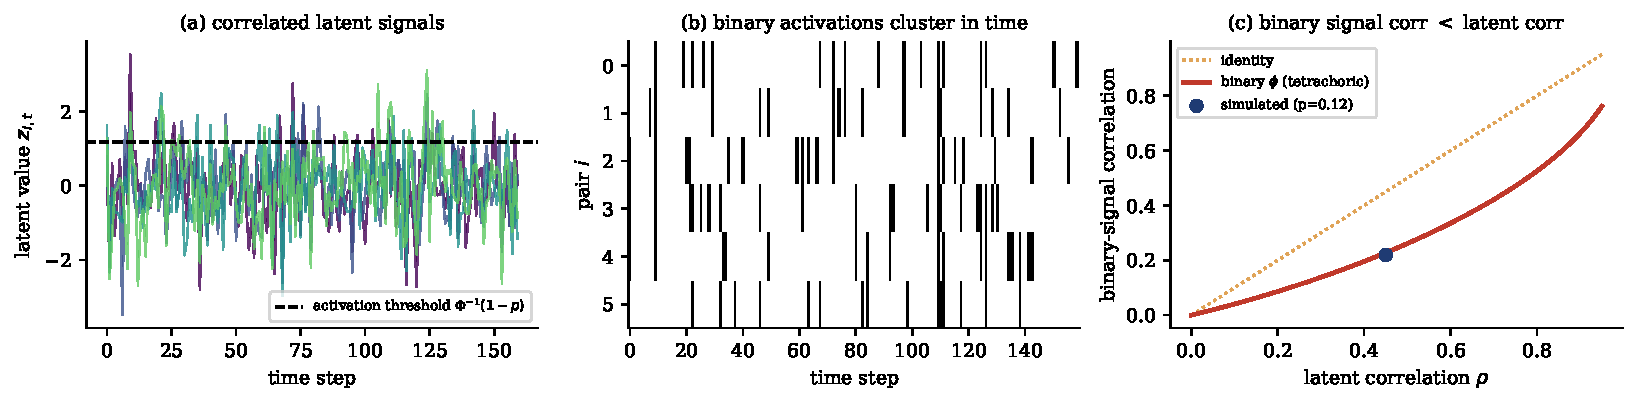
\includegraphics[width=\textwidth]{fig_setup.pdf}
\caption{The generative model. (a) Correlated latent Gaussian drivers and the
activation threshold $\Phi^{-1}(1-p)$. (b) The resulting binary activations
cluster in time. (c) Dichotomization attenuates correlation: the binary
(phi) correlation lies well below the latent correlation that produced it; the
tetrachoric curve predicts the attenuation.}
\label{fig:setup}
\end{figure}

\section{Results}

\subsection{As a PnL diversification discount, $\Neff$'s bias is set by the
return channel}
\label{sec:breadth}

Figure~\ref{fig:breadth} and Tables~\ref{tab:breadth}--\ref{tab:beta} report how
well $\Neff$ predicts the realized PnL effective $N$. Marginally over the
$\beta$ grid the binary-fed formula shows a mean absolute error of $51.7\%$
(bias $+4.1\%$) and the latent-fed one $49.3\%$ (bias $-28.4\%$)---but the
marginal numbers conceal the real structure, which is the $\beta$-dependence in
Table~\ref{tab:beta}. At $\beta=0$, where returns share no factor beyond
co-activation, realized PnL breadth stays close to $N$ and \emph{both} feedings
under-count badly ($-56\%$ binary-fed, $-69\%$ latent-fed). At $\beta=0.9$ both
over-count ($+91\%$ and $+30\%$). The sign of the bias flips between: at the
central $\beta=0.6$ the binary feeding over-counts ($+21.7\%$, MAPE $25.8\%$)
while the latent feeding under-counts ($-16.1\%$, MAPE $32.6\%$). A
signal-level correlation simply does not contain the information ($\beta$) that
determines PnL co-movement, so no feeding of \eqref{eq:neff} can be unbiased
across return regimes.

Two features \emph{are} robust across $\beta$. First, the ordering: the
binary-fed estimate always claims more breadth than the latent-fed one, by a
construction-driven ${\sim}56\%$ (next subsection), with the bias spread
between the two feedings widening from $12.6$pp at $\beta=0$ to $61.4$pp at
$\beta=0.9$ as the realized breadth it is measured against shrinks. Second,
structure barely matters: accuracy degrades little from homogeneous
($51.8\%$) to heterogeneous ($51.5\%$) correlation---the binary attenuation and
the return channel, not correlation heterogeneity, dominate the error.

\begin{figure}[t]
\centering
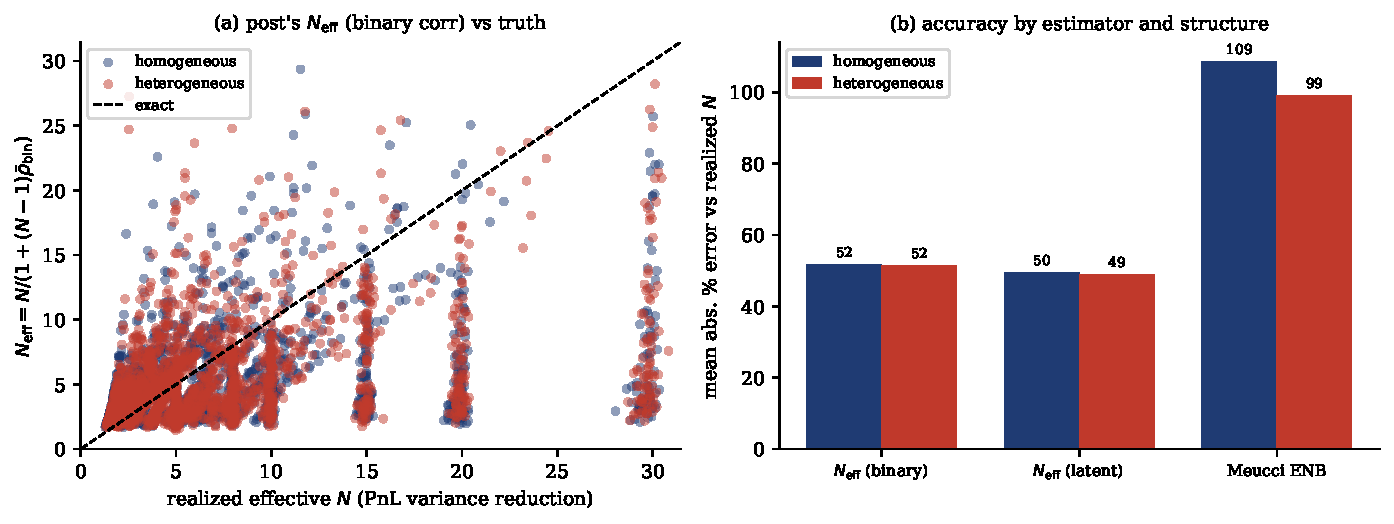
\includegraphics[width=\textwidth]{fig_breadth_accuracy.pdf}
\caption{(a) The shortcut's $\Neff$ (fed binary correlation) versus the realized
PnL effective $N$, all $4{,}000$ portfolios shown (axes span the full data
range). The vertical bands near $N^{\star}\!\approx\!N$ are low-$\beta$
portfolios whose PnL streams are nearly independent. (b) Mean absolute
percentage error by estimator and structure, marginal over the $\beta$ grid.
Meucci's ENB measures a different quantity and diverges far more
(Section~\ref{sec:enb}).}
\label{fig:breadth}
\end{figure}

\begin{table}[t]
\centering
\caption{Accuracy of effective-breadth estimators against the realized
variance-reduction effective $N$ of the PnL streams ($4{,}000$ portfolios,
marginal over the $\beta$ grid). MAPE = mean absolute percentage error; bias is
signed.}
\label{tab:breadth}
\small
\begin{tabular}{lcc@{\hskip 2em}cc@{\hskip 2em}cc}
\toprule
& \multicolumn{2}{c}{Overall} & \multicolumn{2}{c}{Homogeneous} & \multicolumn{2}{c}{Heterogeneous}\\
\cmidrule(lr){2-3}\cmidrule(lr){4-5}\cmidrule(lr){6-7}
Estimator & MAPE & bias & MAPE & bias & MAPE & bias \\
\midrule
$\Neff$ (binary corr.)  & 51.7\% & $+4.1\%$ & 51.8\% & $+2.1\%$ & 51.5\% & $+6.1\%$ \\
$\Neff$ (latent corr.)  & 49.3\% & $-28.4\%$ & 49.5\% & $-31.4\%$ & 49.0\% & $-25.5\%$ \\
Meucci ENB (latent)     & 103.9\% & $+85.1\%$ & 108.6\% & $+89.4\%$ & 99.2\% & $+80.8\%$ \\
\bottomrule
\end{tabular}
\end{table}

\begin{table}[t]
\centering
\caption{The return-factor loading $\beta$ sets the size \emph{and sign} of
$\Neff$'s bias against realized PnL breadth (${\sim}1{,}000$ portfolios per
row). The feeding gap (binary minus latent bias) is the tetrachoric-driven,
$\beta$-robust ordering; its magnitude in percentage points grows with $\beta$
because the realized breadth in the denominator shrinks.}
\label{tab:beta}
\small
\begin{tabular}{ccc@{\hskip 2em}cc@{\hskip 2em}c}
\toprule
& \multicolumn{2}{c}{$\Neff$ (binary corr.)} & \multicolumn{2}{c}{$\Neff$ (latent corr.)} & \\
\cmidrule(lr){2-3}\cmidrule(lr){4-5}
$\beta$ & MAPE & bias & MAPE & bias & spread (pp) \\
\midrule
0.0 & 56.4\% & $-56.4\%$ & 69.0\% & $-69.0\%$ & 12.6 \\
0.3 & 35.7\% & $-33.7\%$ & 55.3\% & $-54.3\%$ & 20.6 \\
0.6 & 25.8\% & $+21.7\%$ & 32.6\% & $-16.1\%$ & 37.7 \\
0.9 & 91.4\% & $+91.4\%$ & 39.3\% & $+30.0\%$ & 61.4 \\
\bottomrule
\end{tabular}
\end{table}

\subsection{The binary/latent distinction is large and predictable}
\label{sec:tetrachoric}

The reason \emph{which} correlation one feeds matters is that dichotomizing
attenuates it. Across our portfolios the mean latent correlation of $0.324$ becomes
a mean binary signal correlation of $0.176$---a median per-portfolio attenuation
ratio of $0.52$, with the binary correlation below the latent one in $98\%$ of
cases. The classical tetrachoric relation predicts the binary correlation from
the latent one and the activation rate to a mean absolute error of just
$0.018$. The practical consequence is direct: feeding $\Neff$ the (smaller)
binary correlation instead of the latent one inflates the estimated effective
count by $+56\%$ on average ($5.19$ vs.\ $3.43$). This inflation depends only on
the activation geometry, not on $\beta$---which is exactly why the binary-fed
estimate sits above the latent-fed one at every $\beta$ in
Table~\ref{tab:beta}. A user of \eqref{eq:neff} who measures correlation on the
signals themselves---the natural thing to do---always claims more
diversification than a latent-correlation user, and overstates the truth
whenever return co-movement is appreciable.

\subsection{The formula is near-exact for the signal streams; the PnL error is
the return channel}
\label{sec:channel}

Two further measurements locate the error. First, judged against the variance
reduction of the \emph{binary signal streams themselves}, the binary-fed
$\Neff$ is essentially exact: $0.022\%$ MAPE across all $4{,}000$ portfolios,
heterogeneous and block structures included. This is close to an algebraic
identity---for equal-variance streams the equal-weight variance-reduction ratio
depends on the correlation matrix only through its mean---so it should be read
as a consistency check, but a useful one: it rules out any contribution of
correlation \emph{heterogeneity} per se to the PnL-stream error. The entire
${\sim}50\%$ PnL error of Table~\ref{tab:breadth} comes from the mismatch
between signal-level and PnL-level correlation, i.e.\ from tetrachoric
attenuation and the return channel $\beta$, not from the equicorrelation
algebra.

Second, the error is concentrated in the weak-correlation regime. At the
central $\beta=0.6$, the binary-fed MAPE falls from $62\%$ in the lowest-$\rho$
bin ($\rho\le0.1$) to $9\%$ for $\rho\in(0.45,0.7]$: when correlation is strong
it dominates both the signal and the PnL structure, and the input mismatch
matters less. (The direction of this $\rho$-dependence is itself
$\beta$-conditional: at $\beta=0$, where realized PnL breadth stays near $N$,
the formula's aggressive discounts make the error \emph{grow} with $\rho$
instead, from $23\%$ to $76\%$.) The uncomfortable reading for practice: in the
regime where a correlation correction seems most affordable---weak-to-moderate
measured correlation---the shortcut is least reliable, and where it is most
accurate the correction is largest.

\subsection{Meucci's ENB answers a different question}
\label{sec:enb}

It is tempting to treat Meucci's ENB as the ``true'' effective number and judge
$\Neff$ against it. Our results caution against this. The ENB diverges from the
realized equal-weight variance reduction by $104\%$ (computed on latent
correlations) to $120\%$ (on return correlations), far more than $\Neff$ does
(Table~\ref{tab:breadth}). This is not a failure of the ENB: it faithfully measures
the number of uncorrelated risk \emph{factors} (the entropy of the eigenvalue
spectrum), which is a different quantity from the variance reduction obtained by a
specific equal-weight combination. The lesson is that ``effective number'' is not
one quantity, and a capacity or diversification claim must name the operational
target. For the equal-weight signal basket that motivates the shortcut, the
variance-reduction $N^{\star}$ is the relevant ground truth, and $\Neff$---for all
its roughness on PnL streams---is far closer to it than the spectral ENB.

\subsection{As a capacity model: the mean load is structurally wrong, and the
$P(\ge1)$ error depends on the feeding}
\label{sec:capacity}

The second use of $\Neff$ is to size execution capacity via
$1-(1-p)^{\Neff}$ and $\mathbb{E}[\text{active}]=\Neff\,p$. The mean-load
identity is wrong by construction: by linearity of expectation the mean number
of simultaneously active signals is $Np$ for \emph{any} correlation
structure---correlation changes the \emph{variance} of the active count, not its
mean. Empirically, $Np$ predicts the simulated mean active count to a MAE of
$0.011$ (sampling noise), whereas $\Neff\,p$ is off by $2.13$ latent-fed
(recovering $0.31\times$ the true load) and $1.87$ binary-fed ($0.44\times$;
Table~\ref{tab:capacity}).

The $P(\ge1\ \text{active})$ heuristic is wrong more subtly: clustering does
reduce the union probability, but less than the heuristic claims, so it
systematically undershoots---and by how much depends on which correlation is
fed. Latent-fed, the MAE is $0.209$ (bias $-0.209$), worse than even the naive
independent-$N$ model ($0.137$); it beats the naive model in only $20\%$ of
portfolios. Binary-fed---the input a practitioner measuring the signals would
actually use---the attenuated correlation yields a larger $\Neff$ and a
prediction much closer to the truth: MAE $0.105$, beating the naive model in
$68\%$ of portfolios. The undershoot is structural in both cases, but the
common practice of quoting the latent-fed numbers alone overstates the
indictment.

The $\rho$-dependence must also be stated precisely. The \emph{absolute error}
of both feedings rises with $\rbar$ in the main batch (Spearman rank
correlation $0.49$ latent-fed and $0.65$ binary-fed, both $p<10^{-200}$), but
the naive model's error rises faster. In the controlled sweep ($N=10$, $p=0.1$;
Figure~\ref{fig:util}) the latent-fed error peaks near $\rho\approx0.3$ and
\emph{crosses below the naive error at $\rho\approx0.5$}: at high correlation
the heuristic beats ignoring correlation, despite its bias. The binary-fed
error sits below the naive error for all $\rho\ge0.1$. By $\rbar$-tercile of
the main batch, the latent-fed\,/\,binary-fed\,/\,naive MAEs are
$0.13/0.04/0.04$ (low), $0.25/0.12/0.13$ (mid), and $0.25/0.15/0.24$ (high).
With three slots, true utilization is $0.491$; the heuristic predicts $0.226$
latent-fed and $0.306$ binary-fed. The heuristic conflates a real effect
(correlation makes the active count \emph{lumpier}, so a fixed slot budget is
sometimes overwhelmed and often idle) with a fall in the \emph{mean} load,
which does not occur.

\begin{table}[t]
\centering
\caption{Execution-capacity predictions vs.\ simulation under both feedings of
$\Neff$. The reference column gives the true $Np$ for the mean-load rows and
the naive independent model $1-(1-p)^N$ for the $P(\ge1)$ row.}
\label{tab:capacity}
\small
\begin{tabular}{lccc}
\toprule
Quantity & $\Neff$ latent-fed & $\Neff$ binary-fed & reference \\
\midrule
Mean active count, MAE                & 2.13 & 1.87 & 0.011\ \ (truth $Np$) \\
Mean active count, ratio to truth     & $0.31\times$ & $0.44\times$ & $1.00\times$\ \ (truth $Np$) \\
$P(\ge1)$, $K{=}1$, MAE               & 0.209 & 0.105 & 0.137\ \ (naive) \\
Slot utilization $K{=}3$ (sim $0.491$) & 0.226 & 0.306 & --- \\
\bottomrule
\end{tabular}
\end{table}

\begin{figure}[t]
\centering
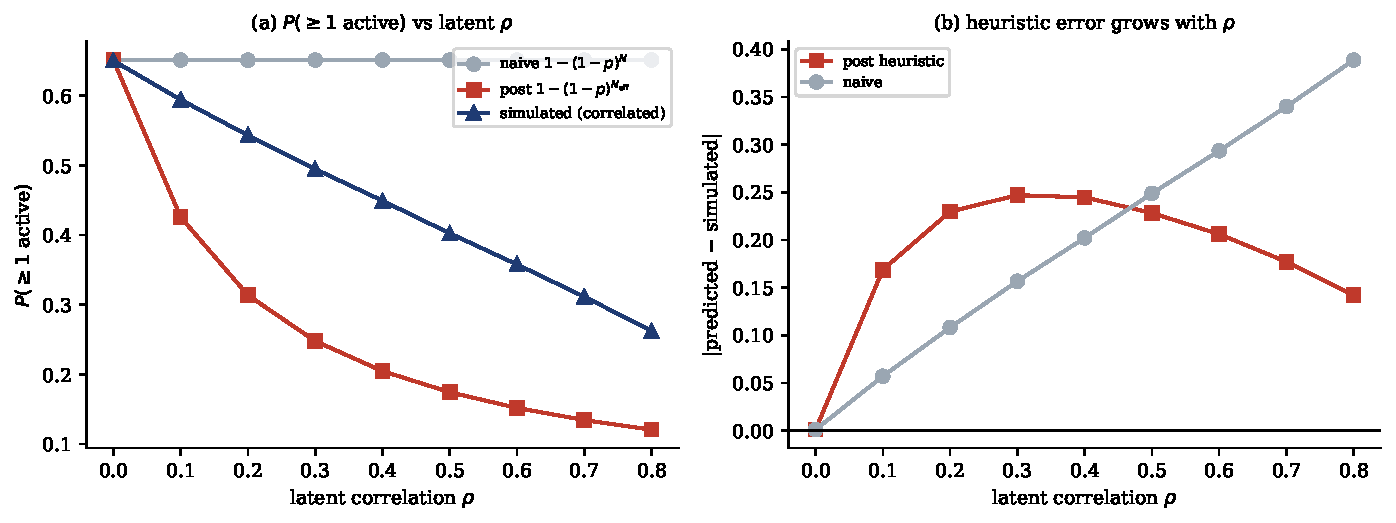
\includegraphics[width=\textwidth]{fig_utilization.pdf}
\caption{Execution-capacity error of $1-(1-p)^{\Neff}$ ($N=10$, $p=0.1$, five
repetitions per $\rho$). (a) Both feedings undershoot the simulated
$P(\ge1\ \text{active})$; the binary-fed prediction lies between the latent-fed
one and the naive model. (b) Absolute errors: the latent-fed error peaks near
$\rho\approx0.3$ and crosses \emph{below} the naive model's error at
$\rho\approx0.5$---at high correlation the heuristic beats ignoring correlation
---while the binary-fed error is below the naive error for all $\rho\ge0.1$.
The error does not grow monotonically with $\rho$; what grows fastest is the
naive model's error.}
\label{fig:util}
\end{figure}

\subsection{The implied ``optimal number of pairs'' is biased low---at a modest
cost}
\label{sec:optimal}

Putting the pieces together, a common application chooses the number of instruments
$N$ that maximizes throughput under a slot budget and a decaying per-instrument
edge. Because the $\Neff$ capacity model undershoots fill rates, it stops adding
instruments too early. Under the homogeneous design point (one slot, $p=0.15$,
$\rho=0.3$, decaying edge), across five independent seeds the simulated optimum
is $N^{\star}_{\text{sim}}=11$--$13$ (median $12$), while the latent-fed
heuristic recommends $N=7$ in every seed (gap $-4$ to $-6$) and the binary-fed
variant $N=9$--$10$ (gap $-2$ to $-4$). Under a genuinely heterogeneous design
(dispersed loadings, three blocks), the simulated optimum is $10$--$15$ (median
$13$) against latent-fed recommendations of $7$--$13$ (gap $-7$ to $0$) and
binary-fed $8$--$15$ (gap $-5$ to $0$).

Two qualifications temper the headline. First, the simulated optimum itself
moves by $\pm2$ across seeds, so single-seed gaps (including the 12-vs-13
homogeneous-vs-heterogeneous contrast in an earlier version of this experiment)
are partly seed noise; we therefore report ranges. Second, the score curve is
flat near its maximum (Figure~\ref{fig:optn}b): trading at the latent-fed
recommendation forfeits on average only $6.9\%$ (homogeneous) and $5.1\%$
(heterogeneous) of attainable throughput, and the binary-fed recommendation
only $1.7\%$ and $1.1\%$. The heuristic stops early, but the cliff it stops
before is shallow. A desk following the formula under-deploys, mildly.

\begin{figure}[t]
\centering
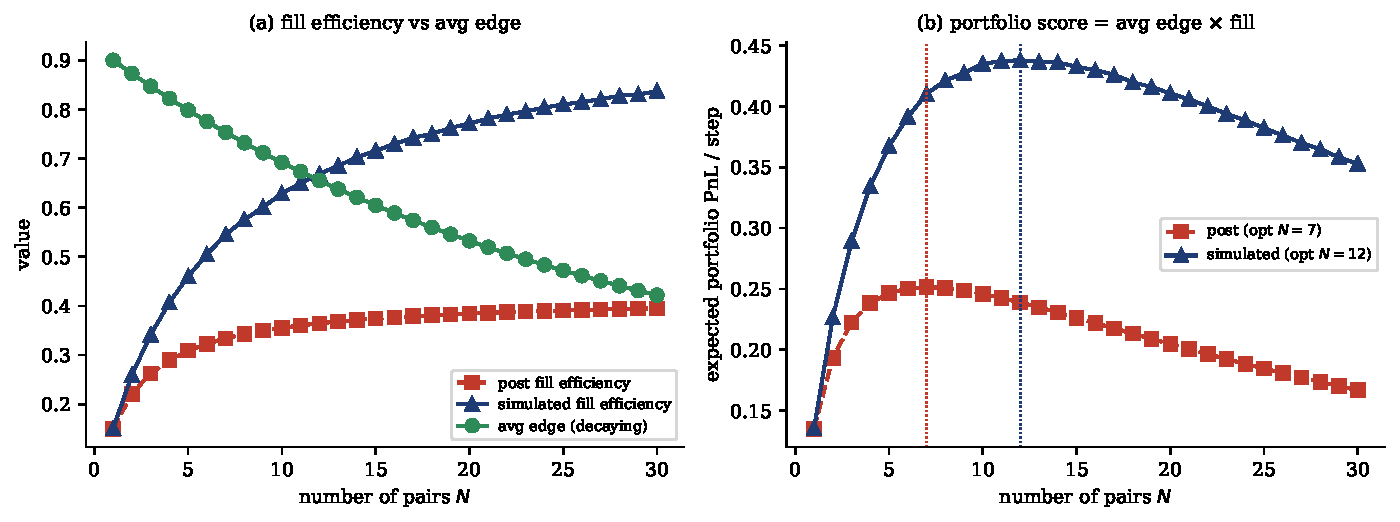
\includegraphics[width=0.85\textwidth]{fig_optimal_n.pdf}
\caption{Throughput vs.\ number of instruments under a slot budget and decaying
edge (homogeneous design, representative seed). The latent-fed heuristic's
score peaks at $N\!=\!7$ and the binary-fed at $N\!=\!9$, vs.\ the simulated
optimum $N\!=\!11$ in this seed (median $12$, range $11$--$13$ across five
seeds). The simulated score curve is flat near its maximum, so the throughput
cost of the early stop is ${\sim}7\%$ (latent-fed) and ${\sim}2\%$
(binary-fed).}
\label{fig:optn}
\end{figure}

\section{Discussion}

The shortcut $\Neff=N/(1+(N-1)\rbar)$ should be split into its two uses, and
each verdict must name the correlation being fed.

As a \emph{diversification discount} for the signal streams themselves it is
essentially exact, and as a PnL discount it is rough at best: its bias is set
by the return-factor loading $\beta$, which no signal-level correlation
contains. Neither feeding is reliably unbiased---the binary-fed version's
near-zero marginal bias ($+4\%$) is an artifact of opposite-sign errors
cancelling across return regimes (Table~\ref{tab:beta}). The defensible default
is the \emph{latent} (or return) correlation, read as a conservative discount:
in our grid it under-counts breadth everywhere except the extreme $\beta=0.9$
corner, and under-counting is the safe direction for risk. Feeding the binary
signal correlation claims ${\sim}56\%$ more breadth by construction and
overstates true diversification precisely when return co-movement is
strong---the dangerous direction. Either way the result should be judged
against equal-weight variance reduction, not the spectral ENB, which measures
factor breadth.

As a \emph{capacity model} the verdict is harsher but should be precise rather
than blanket. The mean-load identity $\mathbb{E}[\text{active}]=\Neff\,p$ is
simply wrong: the truth is $Np$ irrespective of correlation, and the relevant
effect of correlation is on the \emph{dispersion} of the load, which a
correlated-Bernoulli (or directly simulated) model captures and
$1-(1-p)^{\Neff}$ does not. The $P(\ge1)$ heuristic undershoots systematically
at low-to-mid $\rbar$, and its quality depends on the feeding: latent-fed it is
worse than assuming independence; binary-fed it is better than independence in
two out of three portfolios, and its optimal-$N$ recommendation costs only
${\sim}1$--$2\%$ of throughput. If the heuristic is used at all for fill
estimates, it should be fed the binary correlation; load and slot budgets
should be sized from $Np$ and the distribution of the active count.

\section{Limitations}

Our dependence is Gaussian-copula with one factor plus optional blocks; real
signals exhibit tail co-movement and regime-dependent correlation
\citep{cont2001empirical,embrechts2002correlation} that a single $\rbar$ cannot
represent and that would further stress $\Neff$. Our return model
\eqref{eq:returns} ties PnL co-movement to a single constant $\beta$ per
portfolio; real return loadings vary across instruments and time, and our
$\beta$ grid ($0$--$0.9$), while spanning weak to strong co-movement, is itself
a modeling choice. We study equal-weight baskets and a simple slot
orchestrator; capacity-aware weighting, queueing, and priority among signals
are out of scope. Activation is a fixed-threshold binary; graded position
sizing would change the tetrachoric attenuation. Finally we model no
transaction costs, and our ``edge decay'' in the optimal-$N$ exercise is a
stylized assumption, not an empirical estimate. None of these affects the
central structural result---$\mathbb{E}[\text{active}]=Np$---which is exact.

\section{Conclusion}

We tested a popular effective-number shortcut for portfolios of correlated trading
signals against simulated ground truth. As a diversification discount it is
essentially exact for the binary signal streams themselves, but for PnL streams
its accuracy---including the sign of its bias---depends on how strongly returns
co-move beyond co-activation, a quantity ($\beta$) that no signal-level
correlation reveals; the robust, predictable effect is tetrachoric attenuation,
which makes any binary-fed estimate claim ${\sim}56\%$ more breadth than its
latent-fed counterpart. As a model of execution capacity its mean-load
arithmetic is structurally wrong---the mean load is the correlation-free
$Np$---and its $P(\ge1)$ estimate undershoots, badly when fed the latent
correlation (worse than assuming independence) and tolerably when fed the
binary correlation, biasing the implied optimal instrument count low by
$2$--$6$ at a $1$--$7\%$ throughput cost. Use $\Neff$ as a conservative breadth
discount fed the latent or return correlation; size slot budgets from $Np$ and
the distribution of the active count, not from $\Neff$.

\paragraph{Reproducibility.} All experiments are deterministic given the released
seeds; the script \texttt{run\_all.py} regenerates every number and figure, and
\texttt{scripts/check\_paper\_numbers.py} verifies that every number quoted in
this paper matches the generated results. The generative model, the breadth and
capacity measures, and the analysis are provided as an open-source package.

\small
\bibliographystyle{plainnat}
\bibliography{refs}

\end{document}
